% ============================================================
% Final Project Presentation
% Project 14: Structured Document-Level Translation (doctrans)
% Course: CSC15012 - Applications of NLP in Industry
% Student: Le Dinh Minh Quan - 23127460 - 23CNTThuc
% Style mirrors the Project-16 reference deck (Madrid + seahorse).
% ZERO uploaded images: every diagram is TikZ, every chart pgfplots.
% Only optional upload: logo_hcmus.png (guarded by \IfFileExists).
% ============================================================

\documentclass[10pt,aspectratio=169]{beamer}

\mode<presentation>
{
  \usetheme{Madrid}
  \usecolortheme{seahorse}
  \usefonttheme{default}
  \setbeamertemplate{navigation symbols}{}
  \setbeamertemplate{caption}[numbered]
  \setbeamertemplate{footline}[frame number]
}

% ---- Packages ----
\usepackage[english]{babel}
\usepackage[utf8]{inputenc}
\usepackage{amsmath}
\usepackage{graphicx}
\usepackage{booktabs}
\usepackage{xcolor}
\usepackage{hyperref}
\usepackage{xurl}
\usepackage{tikz}
\usepackage{pgfplots}
\pgfplotsset{compat=1.18}
\usetikzlibrary{shapes.geometric, arrows.meta, positioning, fit, backgrounds, shadows}
\usepackage{listings}
\lstset{
  basicstyle=\ttfamily\scriptsize,
  breaklines=true,
  frame=single,
  backgroundcolor=\color{gray!10},
  keywordstyle=\color{blue},
  commentstyle=\color{green!60!black},
  stringstyle=\color{red!70!black},
  showstringspaces=false,
  tabsize=2
}

% ---- HCMUS LOGO ----
% Upload logo_hcmus.png to Overleaf to display the logo (top-right of every slide).
% If the file is missing, no logo is shown (no error).
\IfFileExists{logo_hcmus.png}{\logo{\includegraphics[height=0.7cm]{logo_hcmus.png}}}{}

% ---- TITLE METADATA ----
\title[Project 14: Document-Level Translation]{Project 14: Structured Document-Level Translation}
\subtitle{Structure-Preserving, Context-Aware Machine Translation (\texttt{doctrans})}
\author[Le Dinh Minh Quan]{Le Dinh Minh Quan \\ \small ID: 23127460 -- Class: 23CNTThuc}
\institute[HCMUS]{Vietnam National University Ho Chi Minh City \\ University of Science -- Faculty of Information Technology \\ \small Course: CSC15012 -- Applications of NLP in Industry}
\date{2026}

\begin{document}

% ============================================================
% SLIDE 1: TITLE
% ============================================================
\begin{frame}
  \titlepage
\end{frame}

% ============================================================
% SLIDE 2: OUTLINE
% ============================================================
\begin{frame}{Outline}
\begin{columns}[T]
\begin{column}{0.5\textwidth}
\begin{enumerate}
  \item Business Problem \& Motivation
  \item Proposed NLP Solution \& Success Metrics
  \item System Architecture
  \item Repository \& Tech Stack
  \item Data Overview
  \item Trainable MT Core \& Context (concat-$k$)
  \item Training Workflow (Autopilot)
  \item Evaluation Results
\end{enumerate}
\end{column}
\begin{column}{0.5\textwidth}
\begin{enumerate}
  \setcounter{enumi}{8}
  \item Agentic AI Component (D1--D5)
  \item Example Decision Trace
  \item Deployment
  \item Ethics, Privacy \& Fairness
  \item Monitoring \& Continual Learning
  \item Key Takeaways \& Future Work
  \item Resources \& Thank You
\end{enumerate}
\end{column}
\end{columns}
\end{frame}

% ============================================================
% SLIDE 3: BUSINESS PROBLEM & MOTIVATION
% ============================================================
\begin{frame}{1. Business Problem \& Motivation}
\begin{block}{Context}
Real-world translation operates on \textbf{structured documents} (Markdown, HTML, JSON, plain text), not bare sentences. Raw MT translates the prose but \textbf{corrupts the structure}.
\end{block}

\begin{columns}[T]
\begin{column}{0.5\textwidth}
\textbf{Pain points}
\begin{itemize}
  \item \textbf{Structural corruption}: raw MT eats list markers, translates URLs / placeholders, mangles tables \& code
  \item \textbf{Discourse drift}: sentence-by-sentence loses context (pronouns, formality, terminology)
  \item \textbf{Post-edit cost}: engineers fix structure, not language
\end{itemize}
\end{column}
\begin{column}{0.5\textwidth}
\textbf{Stakeholders}
\begin{itemize}
  \item Localization engineers (JSON/HTML bundles)
  \item Documentation writers (byte-stable French docs)
  \item Developers / i18n owners (REST API in CI/CD)
  \item MT researchers (does context actually help?)
\end{itemize}
\end{column}
\end{columns}
\end{frame}

% ============================================================
% SLIDE 4: PROPOSED NLP SOLUTION + SUCCESS METRICS
% ============================================================
\begin{frame}{2. Proposed NLP Solution \& Success Metrics}
\begin{block}{Solution: the localization spine}
\textbf{parse $\rightarrow$ mask $\rightarrow$ translate-with-context $\rightarrow$ restore $\rightarrow$ reassemble $\rightarrow$ validate.} One principle: \emph{the model never sees structure, and the structure layer never sees the model.} The only trainable stage is the MT core (\texttt{m2m100}); everything else is deterministic code.
\end{block}

\begin{table}[h]
\centering\small
\begin{tabular}{lll}
\toprule
\textbf{Type} & \textbf{Metric} & \textbf{Target} \\
\midrule
Business  & Localization post-edit (needs-review) rate & Reduce vs.\ manual \\
Business  & Structurally-broken output rate            & $\approx$ 0\% (hard gates) \\
Technical & chrF (headline MT quality)                 & Beat all baselines \\
Technical & Placeholder-Retention Rate (PHR)           & $=1.0$ (hard) \\
Technical & Structure-Preservation Score (SPS)         & $=1.0$ target \\
\bottomrule
\end{tabular}
\end{table}

\textbf{Result preview} (verified offline / synthetic-spine seed): dictionary MT chrF \textbf{$\sim$82} vs.\ identity floor \textbf{$\sim$21}; document-level \textbf{d-chrF $\sim$81} at \textbf{SPS = 1.0}, \textbf{PHR = 1.0}. Full fine-tuned MT numbers come from the Colab H100 run.
\end{frame}

% ============================================================
% SLIDE 5: SYSTEM ARCHITECTURE (TikZ)
% ============================================================
\begin{frame}{3. System Architecture (Two Artifacts, Two Lifecycles)}
\centering
\resizebox{\linewidth}{!}{%
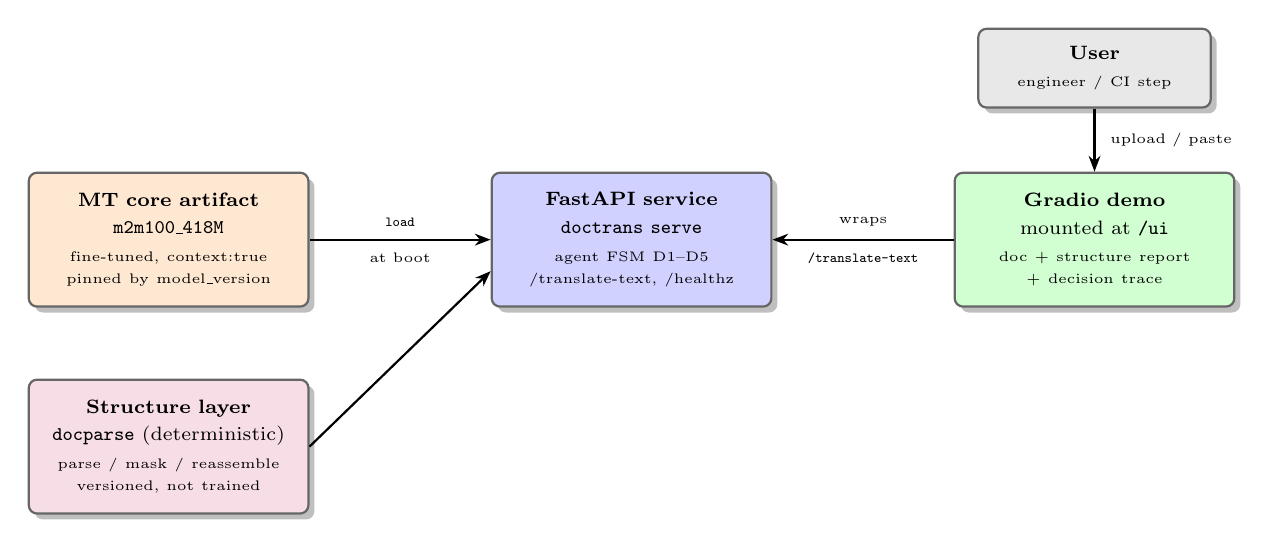
\begin{tikzpicture}[
  node distance=0.9cm and 2.3cm,
  box/.style={rectangle, draw=black!60, rounded corners=3pt, thick,
              text width=3.2cm, minimum height=1.7cm, align=center,
              inner sep=5pt, font=\scriptsize, drop shadow},
  modelbox/.style={box, fill=orange!18},
  structbox/.style={box, fill=purple!13},
  apibox/.style={box, fill=blue!18},
  uibox/.style={box, fill=green!18},
  userbox/.style={box, fill=gray!18, text width=2.6cm, minimum height=1.0cm},
  arrow/.style={-{Stealth[length=2mm]}, thick}
]

\node[modelbox] (mt) {%
  \textbf{MT core artifact}\\[2pt]
  \texttt{m2m100\_418M}\\[2pt]
  {\tiny fine-tuned, context:true}\\
  {\tiny pinned by model\_version}
};
\node[structbox, below=of mt] (struct) {%
  \textbf{Structure layer}\\[2pt]
  \texttt{docparse} (deterministic)\\[2pt]
  {\tiny parse / mask / reassemble}\\
  {\tiny versioned, not trained}
};
\node[apibox, right=of mt] (api) {%
  \textbf{FastAPI service}\\[2pt]
  \texttt{doctrans serve}\\[2pt]
  {\tiny agent FSM D1--D5}\\
  {\tiny /translate-text, /healthz}
};
\node[uibox, right=of api] (ui) {%
  \textbf{Gradio demo}\\[2pt]
  mounted at \texttt{/ui}\\[2pt]
  {\tiny doc + structure report}\\
  {\tiny + decision trace}
};
\node[userbox, above=0.8cm of ui] (user) {%
  \textbf{User}\\[2pt]
  {\tiny engineer / CI step}
};

\draw[arrow] (mt.east) -- node[above=1pt, font=\tiny, midway] {\texttt{load}} node[below=1pt, font=\tiny, midway] {at boot} (api.west);
\draw[arrow] (struct.east) -- ([yshift=-4mm]api.west);
\draw[arrow] (ui.west) -- node[above=1pt, font=\tiny, midway] {wraps} node[below=1pt, font=\tiny, midway] {\texttt{/translate-text}} (api.east);
\draw[arrow] (user) -- node[right=2pt, font=\tiny] {upload / paste} (ui);
\end{tikzpicture}%
}

\vspace{0.2cm}
\scriptsize \textbf{Separation of concerns}: the deterministic structure layer and the pinned MT core artifact are both loaded by FastAPI; the Gradio demo wraps \texttt{/translate-text}. Two artifacts, two lifecycles. Fully \emph{deployable} (API + UI + Docker + Colab) but \emph{not} hosted at a live public URL.
\end{frame}

% ============================================================
% SLIDE 6: REPOSITORY & TECH STACK
% ============================================================
\begin{frame}[fragile]{4. Repository Structure \& Tech Stack}
\begin{columns}[T]
\begin{column}{0.55\textwidth}
\textbf{GitHub repo} (public, MIT) \\
\scriptsize \url{https://github.com/ledinhminhquan/14_Document_Level_Translation}

\vspace{0.15cm}
\begin{lstlisting}[basicstyle=\ttfamily\tiny]
14_Document_Level_Translation/
|-- src/doctrans/
|   |-- config.py  cli.py  logging_utils.py
|   |-- data/        # opus-100/news_commentary + seed
|   |-- models/      # model registry
|   |-- docparse/    # THE STRUCTURE LAYER
|   |   |-- segment.py  mask.py  router.py
|   |   |-- {markdown,html,json,plain}_doc.py
|   |   +-- structure_score.py  # SPS
|   |-- mt/          # translator (m2m100) + context (concat-k)
|   |-- training/    # train_mt, evaluate, tune, metrics
|   |-- agent/       # D1-D5 FSM + tools + ToolTrace
|   |-- api/         # FastAPI + Gradio
|   |-- analysis/  autoreport/  monitoring/
|   |-- automation/autopilot.py
|   +-- grading/checklist.py
|-- configs/  docs/ (15 md)  tests/  notebooks/
|-- app/  deploy/  scripts/  sample_data/
|-- Dockerfile, docker-compose.yml, Makefile
+-- README.md, pyproject.toml, LICENSE (MIT)
\end{lstlisting}
\end{column}
\begin{column}{0.45\textwidth}
\textbf{Tech stack}
\begin{itemize}\small
  \item Python 3.12, Git + GitHub
  \item PyTorch + Transformers (\texttt{Seq2SeqTrainer})
  \item HF Datasets, Accelerate
  \item \textbf{\texttt{m2m100\_418M}} ($\sim$418M, MIT)
  \item \texttt{sacrebleu} + \texttt{evaluate} (chrF/BLEU)
  \item Structure: \texttt{markdown-it-py}, \texttt{beautifulsoup4}, \texttt{python-docx} (all optional)
  \item FastAPI + Uvicorn, Gradio at \texttt{/ui}
  \item Docker + docker-compose; HF Space-ready
  \item NVIDIA H100 80GB (auto-adapts A100/L4/T4)
\end{itemize}
\textbf{Reuse}: MT plumbing (translator, training loop, pure-python metrics) reused from sibling \textbf{P13 \texttt{s2st}}.
\end{column}
\end{columns}
\end{frame}

% ============================================================
% SLIDE 7: DATA OVERVIEW
% ============================================================
\begin{frame}{5. Data Overview}
\begin{columns}[T]
\begin{column}{0.52\textwidth}
\textbf{Honest data constraint}: \textbf{no HF corpus} provides Markdown/HTML/JSON-structured parallel documents, and none provides clean en$\leftrightarrow$fr data with document-boundary metadata.
\begin{itemize}\small
  \item MT core fine-tuned on real sentence pairs
  \item Document context reconstructed from row-adjacency
  \item \textbf{Structure is 100\% synthetic} (real pairs wrapped in Markdown/HTML/JSON) + an offline seed
\end{itemize}

\textbf{Preprocessing}
\begin{itemize}\small
  \item Streaming probes (\texttt{streaming=True}) -- never download multi-GB files
  \item Left-truncate context, never the current sentence
  \item Splits: opus-100 = 1.0M / 2.0K / 2.0K (seed=42)
\end{itemize}
\end{column}
\begin{column}{0.48\textwidth}
\textbf{Datasets \& models (verified on HF Hub)}
\begin{table}[h]
\centering\scriptsize
\begin{tabular}{lll}
\toprule
\textbf{Asset} & \textbf{Role} & \textbf{License} \\
\midrule
\texttt{opus-100} (en-fr)        & MT fine-tune (1M) & \textbf{[FLAG]} \\
\texttt{news\_commentary}         & doc context (209.5K) & \textbf{[FLAG]} \\
\texttt{iwslt2017} (en-fr)       & context alt & \textbf{CC-BY-NC-ND} \\
\texttt{para\_crawl} (enfr)       & permissive sent. & CC0 \\
\texttt{m2m100\_418M}             & MT core (default) & MIT \\
\texttt{nllb-200-distilled}      & stronger (eval) & \textbf{CC-BY-NC} \\
\bottomrule
\end{tabular}
\end{table}
\scriptsize \textbf{License hygiene}: clean path = \texttt{m2m100\_418M} (MIT) + offline seed. Non-commercial (NLLB, IWSLT) flagged, used as research/eval only; unknown-license corpora treated as research/educational. No flag is silently ``upgraded''.
\end{column}
\end{columns}
\end{frame}

% ============================================================
% SLIDE 8: TRAINABLE MT CORE + CONTEXT
% ============================================================
\begin{frame}{6. Trainable MT Core \& Document Context (concat-$k$)}
\begin{columns}[T]
\begin{column}{0.5\textwidth}
\textbf{MT core ladder} (only trainable stage)
\begin{table}[h]
\centering\scriptsize
\begin{tabular}{llc}
\toprule
\textbf{Model} & \textbf{License} & \textbf{Pos.} \\
\midrule
\textbf{\texttt{m2m100\_418M}} (default) & MIT & \textbf{1024} \\
\texttt{mbart-large-50-mmt} & MIT (flag) & 1024 \\
\texttt{opus-mt-en-fr} (lite) & Apache-2.0 & 512 \\
\texttt{nllb-200-distilled} & CC-BY-NC (flag) & 1024 \\
\texttt{madlad400-3b} (zero-shot) & Apache-2.0 & 512 \\
\bottomrule
\end{tabular}
\end{table}
\scriptsize Default \texttt{m2m100\_418M}: MIT (clean), 1024 positions = headroom for prepended context, simple \texttt{src\_lang} + \texttt{forced\_bos\_token\_id} API, reuses P13 plumbing.
\end{column}
\begin{column}{0.5\textwidth}
\textbf{Document context = concat-$k$}
\begin{itemize}\small
  \item Prepend $k$ previous source sentences, joined by a special \texttt{<BRK>} token
  \item Train to output \textbf{only} the current target (\texttt{k-to-1} recipe)
  \item Default \textbf{$k=2$, source-side}; context left-truncated so the current sentence is never cut
  \item Architecture-free; the 1024-position budget makes $k$=2--3 comfortable (Marian's 512 limits it to $k\approx$1--2)
\end{itemize}

\textbf{Baselines (floors to beat)}
\begin{itemize}\small
  \item Identity (copy-source) -- absolute floor
  \item Dictionary lookup -- offline / no-torch floor
  \item Zero-shot MT -- the un-fine-tuned base
\end{itemize}
\end{column}
\end{columns}
\end{frame}

% ============================================================
% SLIDE 9: TRAINING WORKFLOW (AUTOPILOT)
% ============================================================
\begin{frame}{7. Training Workflow -- One-Button Autopilot (Colab H100)}
\centering
\begin{tikzpicture}[
  node distance=0.18cm,
  step/.style={rectangle, draw=black!60, rounded corners=2pt, thick,
              minimum width=11.8cm, minimum height=0.55cm, align=center, font=\scriptsize},
  setup/.style={step, fill=gray!15},
  train/.style={step, fill=orange!15},
  eval/.style={step, fill=blue!15},
  deploy/.style={step, fill=green!15},
  arrow/.style={-{Stealth[length=1.8mm]}, thick}
]
\node[setup] (s1) {\textbf{1. Setup (Colab)}: mount Drive, set \texttt{DOCTRANS\_*\_DIR} + \texttt{HF\_HOME}, GPU auto-profile (H100/A100/L4/T4), Colab-safe install};
\node[setup, below=of s1] (s2) {\textbf{2. Data}: streaming probes of \texttt{opus-100} + \texttt{news\_commentary} (en-fr); build concat-$k$ windows from per-article ids};
\node[train, below=of s2] (s3) {\textbf{3. Baseline}: dictionary MT + identity floor (instant, CPU) -- establishes the floor to beat};
\node[train, below=of s3] (s4) {\textbf{4. Train MT core}: \texttt{m2m100\_418M} fine-tune, \texttt{Seq2SeqTrainer}, concat-$k$ ($k$=2, \texttt{<BRK>}), bf16/tf32, resume-safe};
\node[eval, below=of s4] (s5) {\textbf{5. Evaluate}: chrF / BLEU / d-chrF + SPS (struct $\times$ markup $\times$ PHR); 2$\times$2 sentence-vs-context ablation};
\node[eval, below=of s5] (s6) {\textbf{6. Tune + analysis}: hyperparameter sweep; error analysis + latency benchmark (privacy-preserving, metadata-only)};
\node[deploy, below=of s6] (s7) {\textbf{7. Auto-gen}: \texttt{report\_pdf} (PDF) + \texttt{slides\_pptx} (deck) from versioned JSON artifacts};
\node[deploy, below=of s7] (s8) {\textbf{8. Grade + bundle}: rubric self-check (\texttt{grading/checklist.py}) + submission zip};
\foreach \a/\b in {s1/s2,s2/s3,s3/s4,s4/s5,s5/s6,s6/s7,s7/s8}
  \draw[arrow] (\a) -- (\b);
\end{tikzpicture}

\vspace{0.15cm}
\scriptsize \textbf{Single Run-All} on Colab H100 80GB. \textbf{Resume-safe} (\texttt{get\_last\_checkpoint}); survives disconnects. \textbf{GPU auto-adapt} (\texttt{bf16=torch.cuda.is\_bf16\_supported()}; T4 $\rightarrow$ fp16). \textbf{Offline-degradable}: CI runs the same pipeline on the dictionary/identity baselines over the seed (green on CPU).
\end{frame}

% ============================================================
% SLIDE 10: EVALUATION RESULTS
% ============================================================
\begin{frame}{8. Evaluation Results -- Verified Offline / Synthetic-Spine}
\begin{columns}[T]
\begin{column}{0.52\textwidth}
\textbf{Headline = chrF, reported jointly with SPS}
\begin{table}[h]
\centering\scriptsize
\begin{tabular}{lcc}
\toprule
\textbf{System / metric} & \textbf{Offline} & \textbf{Role} \\
\midrule
Identity (copy-source) chrF & $\sim$21 & absolute floor \\
Dictionary MT chrF          & $\sim$82 & offline lexical floor \\
Document-level chrF (d-chrF) & $\sim$81 & full structure fidelity \\
\textbf{SPS}                 & \textbf{1.0} & struct$\times$markup$\times$PHR \\
\textbf{PHR}                 & \textbf{1.0} & D4 HARD gate \\
\bottomrule
\end{tabular}
\end{table}
\scriptsize A translation that wins chrF but breaks a table or drops a placeholder is a \textbf{failure}, so text quality and structure fidelity are reported together. \textbf{SPS = 1.0} because the model never sees structure and reassembly is the inverse of parsing (D1 round-trip identity). Full fine-tuned MT numbers come from the Colab H100 run.

\vspace{0.1cm}
\scriptsize \textbf{2$\times$2 ablation} isolates fine-tuning vs.\ context. \textbf{Honest caveat}: concat-$k$ can underperform sentence-level on raw chrF when doc-parallel data is scarce, while still fixing discourse cases -- so we report ContraPro-style accuracy + term-consistency, not just $n$-gram scores.
\end{column}
\begin{column}{0.48\textwidth}
\centering
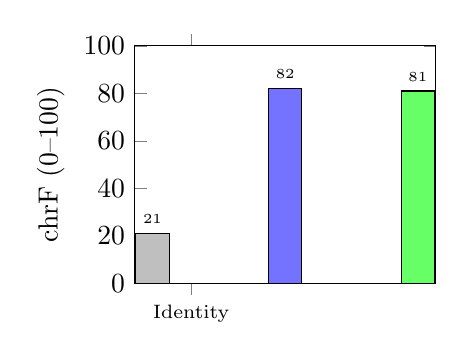
\begin{tikzpicture}
\begin{axis}[
  ybar, width=5.4cm, height=4.6cm,
  ymin=0, ymax=100,
  symbolic x coords={Identity, Dict-MT, d-chrF},
  xtick=data,
  ylabel={chrF (0--100)},
  nodes near coords, every node near coord/.append style={font=\tiny},
  bar width=12pt,
  enlarge x limits=0.3,
  ytick={0,20,40,60,80,100},
  x tick label style={font=\scriptsize}
]
\addplot[fill=gray!50]   coordinates {(Identity,21)};
\addplot[fill=blue!55]   coordinates {(Dict-MT,82)};
\addplot[fill=green!60]  coordinates {(d-chrF,81)};
\end{axis}
\end{tikzpicture}\\
\tiny chrF on the offline seed: dictionary MT and document-level d-chrF both clear the identity floor at \textbf{SPS = 1.0}.
\end{column}
\end{columns}
\end{frame}

% ============================================================
% SLIDE 11: AGENTIC AI COMPONENT (D1-D5 FSM)
% ============================================================
\begin{frame}{9. Agentic AI Component -- Deterministic FSM (D1--D5)}
\centering
\begin{tikzpicture}[
  node distance=0.16cm,
  step/.style={rectangle, draw=black!60, rounded corners=2pt, thick,
              text width=11.4cm, minimum height=0.55cm, align=center, font=\scriptsize,
              inner sep=4pt},
  d1/.style={step, fill=gray!15},
  d2/.style={step, fill=blue!15},
  d3/.style={step, fill=orange!15},
  d4/.style={step, fill=red!12},
  d5/.style={step, fill=green!15},
  arrow/.style={-{Stealth[length=2mm]}, thick}
]
\node[d1] (a1) {\textbf{D1 -- Format detect + parse} (\textit{tool}): ext $\rightarrow$ MIME $\rightarrow$ content sniff; \textbf{round-trip identity} \texttt{reserialize(parse(x))==x}};
\node[d2, below=of a1] (a2) {\textbf{D2 -- Segment + mask} (\textit{decision}): skip if letter-ratio $<$ 0.30; mask code/URLs/placeholders as reversible \texttt{[[PHn]]} sentinels};
\node[d3, below=of a2] (a3) {\textbf{D3 -- Translate with $k$ context} (\textit{multi-step reasoning + tool}): concat-$k$ MT; reject empty / length-ratio outside $[0.4,3.0]$};
\node[d4, below=of a3] (a4) {\textbf{D4 -- Verify gate} (\textit{decision}): \textbf{placeholder-retention HARD} (each \texttt{[[PHn]]} back once) + back-translation chrF $\geq 0.30$ (soft)};
\node[d5, below=of a4] (a5) {\textbf{D5 -- Reassemble + validate} (\textit{tool}): unmask 1:1 $\rightarrow$ slot leaves into untouched skeleton $\rightarrow$ structure-signature match + re-parse};
\foreach \a/\b in {a1/a2,a2/a3,a3/a4,a4/a5}
  \draw[arrow] (\a) -- (\b);
\draw[arrow, dashed, color=red!70] (a4.west) to[bend left=55] node[left, font=\tiny] {fail: re-translate $\leq N{=}2$} (a3.west);
\end{tikzpicture}

\vspace{0.12cm}
\scriptsize \textbf{Deterministic} (same input + model $\rightarrow$ same path + audit trace). Every action is a \textbf{tool} behind one signature ($\rightarrow$ \texttt{ToolTrace}): \textbf{multi-step reasoning} (D3), \textbf{tool usage} (D1/D3/D5), \textbf{decision-making} on intermediate outputs (D2/D4). Budgets are finite ($N{=}2$, $M{=}1$) so termination is guaranteed. Optional Anthropic LLM ``brain'' is \textbf{OFF by default} (advisory terminology note only -- never edits text/structure/placeholders).
\end{frame}

% ============================================================
% SLIDE 12: THE FIVE GATES + EXAMPLE TRACE
% ============================================================
\begin{frame}[fragile]{10. The Five Gates \& an Example Decision Trace}
\begin{columns}[T]
\begin{column}{0.4\textwidth}
\textbf{Hard checks \& fail actions}
\begin{table}[h]
\centering\tiny
\begin{tabular}{ll}
\toprule
\textbf{Gate} & \textbf{HARD check} \\
\midrule
D1 & round-trip identity \\
D2 & masks balanced (1:1) \\
D3 & length-ratio $[0.4,3.0]$ \\
\textbf{D4} & \textbf{placeholder-retention} \\
D5 & structure-signature match \\
\bottomrule
\end{tabular}
\end{table}
\scriptsize \textbf{D4 placeholder-retention is the one non-negotiable HARD gate}: a translation that drops or duplicates a sentinel can never ship. On any failure: re-translate ($N{=}2$) / repair ($M{=}1$), then \textbf{fail-soft} -- flag for review and keep the source.
\end{column}
\begin{column}{0.6\textwidth}
\begin{lstlisting}[basicstyle=\ttfamily\tiny]
Input (sample.md):
  "# Welcome, {user}\nSee the [docs](https://...)."
D1 parse : fmt=markdown; round-trip identity OK
D2 mask  : "Welcome, [[PH0]]" ; "See the [[PH1]]docs[[PH2]]."
           map={PH0:"{user}", PH1:"[", PH2:"](https://...)"}
D3 trans : "Bienvenue, [[PH0]]" ; "Consultez la [[PH1]]docs[[PH2]]."
           length-ratio in [0.4,3.0] -> OK
D4 verify: PH retention {PH0,PH1,PH2} each once -> HARD PASS
           back-translation chrF=0.71 (>=0.30) -> PASS
D5 reasm : unmask 1:1 -> structure-signature match -> PASS
Output (sample.fr.md): structure byte-stable, PH intact
  action=OK, SPS=1.0, PHR=1.0, model_used=m2m100:context
\end{lstlisting}
\scriptsize Every API response returns this \texttt{ToolTrace}, so a reviewer can replay exactly why a document passed, was flagged, or fell back to source.
\end{column}
\end{columns}
\end{frame}

% ============================================================
% SLIDE 13: DEPLOYMENT
% ============================================================
\begin{frame}[fragile]{11. Deployment -- Four Formats}
\begin{columns}[T]
\begin{column}{0.52\textwidth}
\textbf{All four delivered in the repo}
\begin{itemize}\small
  \item \textbf{REST API} (FastAPI): \texttt{POST /translate-text}, \texttt{POST /translate-document}, \texttt{GET /healthz}, \texttt{GET /version}
  \item \textbf{CLI}: \texttt{doctrans serve / train-mt / evaluate / demo-agent / translate / autopilot}
  \item \textbf{Docker}: \texttt{Dockerfile} + \texttt{docker-compose.yml}; same image runs locally and as a HF Space
  \item \textbf{Colab autopilot}: one-button H100 notebook
\end{itemize}
\scriptsize \textbf{Honest status}: fully \emph{deployable} but \emph{not} hosted at a live public URL.
\end{column}
\begin{column}{0.48\textwidth}
\textbf{Multipart gating} (a load-bearing P05/P13 lesson)
\begin{lstlisting}[basicstyle=\ttfamily\tiny]
try:
    import multipart        # python-multipart
    HAS_MULTIPART = True
except ImportError:
    HAS_MULTIPART = False
# /translate-document registered only if present
# /translate-text, /healthz, /version always boot
\end{lstlisting}
\scriptsize \texttt{UploadFile}/\texttt{File()} routes hard-require \texttt{python-multipart}; the document route is gated so the core service never fails to boot over an optional dependency.

\vspace{0.1cm}
\scriptsize \textbf{Offline degradation \& versioning}: every heavy import is lazy; parsers fall back native $\rightarrow$ regex $\rightarrow$ plain and MT falls back to the dictionary translator. \texttt{model\_version} is pinned at startup and surfaced via \texttt{/version}.
\end{column}
\end{columns}
\end{frame}

% ============================================================
% SLIDE 14: ETHICS, PRIVACY & FAIRNESS
% ============================================================
\begin{frame}{12. Ethics, Privacy \& Fairness}
\begin{columns}[T]
\begin{column}{0.5\textwidth}
\textbf{Stance: a localization aid, not an autonomous translator}
\begin{itemize}\small
  \item Structure-breaking / low-confidence output is \textbf{flagged for human review}, never presented as final
  \item \textbf{Fail-soft}: keep the \emph{source} rather than emit a corrupted translation -- silence-with-source beats a confident wrong answer
\end{itemize}

\textbf{Privacy}
\begin{itemize}\small
  \item Local-first, offline-capable (no network, no torch with the seed)
  \item \textbf{Metadata-only} logging: format, segment count, decision trace, SPS, latency -- \textbf{never} document content
  \item Optional LLM brain OFF by default (advisory note only)
\end{itemize}
\end{column}
\begin{column}{0.5\textwidth}
\textbf{Risks \& mitigations}
\begin{table}[h]
\centering\tiny
\begin{tabular}{ll}
\toprule
\textbf{Risk} & \textbf{Mitigation} \\
\midrule
Mistranslation harm & D4 back-translation + length-ratio; advisory, reviewed \\
Structure / PH corruption & HARD gates D1/D4/D5; repair then fail-soft \\
Bias across langs/domains & concat-$k$ context; reported per-domain \\
License misuse & per-asset flags; clean m2m100 (MIT) + seed \\
Over-trust / automation bias & UI/report surface the decision trace \\
Privacy & metadata-only logging; bodies never retained \\
\bottomrule
\end{tabular}
\end{table}
\scriptsize \textbf{Accountability}: each of the five decisions emits a \texttt{ToolTrace}; a human reviewer is the final authority on any flagged document. The structure layer is deterministic, versioned code -- auditable and not subject to model drift.
\end{column}
\end{columns}
\end{frame}

% ============================================================
% SLIDE 15: MONITORING & CONTINUAL LEARNING
% ============================================================
\begin{frame}{13. Monitoring \& Continual Learning}
\begin{columns}[T]
\begin{column}{0.5\textwidth}
\textbf{Two artifacts, two lifecycles}: the MT core is re-fine-tuned on a loop; the structure layer is deterministic code -- versioned, never trained.

\vspace{0.1cm}
\textbf{Re-fine-tune loop (MT core only)}
\begin{enumerate}\small
  \item \textbf{Collect} flagged D3/D4/D5 segments + human references (where the model is weakest)
  \item \textbf{Build context}: re-apply concat-$k$ ($k$=2, source-side)
  \item \textbf{Train}: \texttt{Seq2SeqTrainer}, resume-safe, from the current checkpoint
  \item \textbf{Gate}: promote only if the \textbf{chrF non-regression gate} passes
  \item \textbf{Promote}: passing checkpoints become a new \texttt{model\_version}
\end{enumerate}
\end{column}
\begin{column}{0.5\textwidth}
\textbf{Operational monitor-log signals} (metadata-only)
\begin{table}[h]
\centering\scriptsize
\begin{tabular}{lc}
\toprule
\textbf{Signal} & \textbf{Drift} \\
\midrule
needs-review rate (D3/D4/D5 flags) & up = bad \\
mean SPS (struct$\times$markup$\times$PHR) & down = bad \\
latency (context / retry creep) & up = watch \\
\bottomrule
\end{tabular}
\end{table}
\scriptsize Rising needs-review \emph{and} falling SPS together is the canonical drift signal $\rightarrow$ start a new collect step.

\vspace{0.1cm}
\scriptsize \textbf{Observability}: the per-request \texttt{ToolTrace} answers ``why did \emph{this} document fail?''. Because the structure layer is deterministic, any structure failure is fully reproducible and fixed in code under a new structure-layer version -- never by retraining.
\end{column}
\end{columns}
\end{frame}

% ============================================================
% SLIDE 16: KEY TAKEAWAYS & FUTURE WORK
% ============================================================
\begin{frame}{14. Key Takeaways \& Future Work}
\textbf{Key takeaways}
\begin{itemize}\small
  \item Complete end-to-end NLP system: training $\rightarrow$ evaluation $\rightarrow$ deployment $\rightarrow$ monitoring
  \item Core idea: an \textbf{opaque-sentinel structure layer} + a \textbf{trainable MT core}, gated by a deterministic \textbf{D1--D5 FSM} $\Rightarrow$ byte-stable structure + document-level context
  \item Verified offline: dictionary MT chrF \textbf{$\sim$82} vs identity \textbf{$\sim$21}; d-chrF \textbf{$\sim$81} at \textbf{SPS = 1.0}, \textbf{PHR = 1.0}; full MT numbers from the Colab H100 run
  \item \textbf{Honest confidence story}: fail-soft, human-in-the-loop, per-asset license flags, metadata-only logging
  \item Reproducible offline: dictionary + seed docs run the whole pipeline with no torch / no network (CI green on CPU)
\end{itemize}

\textbf{Future work}
\begin{enumerate}\small
  \item Stronger doc-parallel data for concat-$k$; richer DOCX / PPTX / XLIFF parsers
  \item More language pairs via the same localization spine
  \item Learned segment-skip + per-domain terminology memory
  \item Token-level explainability + a drift dashboard with canary promotion of new model versions
\end{enumerate}
\end{frame}

% ============================================================
% SLIDE 17: RESOURCES & THANK YOU (Final slide)
% ============================================================
\begin{frame}{15. Project Resources \& Thank You}
\begin{block}{Source code (public, MIT)}
\centering
\large \textbf{\url{https://github.com/ledinhminhquan/14_Document_Level_Translation}}
\end{block}

\textbf{Key resources}
\begin{itemize}\scriptsize
  \item \textbf{GitHub repo}: \url{https://github.com/ledinhminhquan/14_Document_Level_Translation}
  \item \textbf{MT core (HF Hub)}: \texttt{facebook/m2m100\_418M} (MIT, 1024 positions) -- fine-tuned via the Colab H100 autopilot notebook
  \item \textbf{Deployment surface}: FastAPI REST API + Gradio demo (\texttt{doctrans serve --ui}), Docker / docker-compose, HF Space-ready image (offline-degradable). Fully deployable; \emph{not} hosted at a live public URL.
  \item \textbf{Reproduce offline}: \texttt{doctrans evaluate --fast} / \texttt{doctrans demo-agent --fast} -- no GPU, no downloads
\end{itemize}

\vspace{0.3cm}
\centering
\Large\textbf{Thank you for your attention!}\\[0.2cm]
\normalsize Le Dinh Minh Quan -- 23127460 -- 23CNTThuc \\
\small CSC15012 -- Applications of NLP in Industry -- 2026
\end{frame}

\end{document}
